%begin module arc-length-derivation-parametric
{% scoping block for the following command:
%Calculator input: plotCurve{}(t, 8 t^{4}-40 t^{3}+70 t^{2}-50 t+13, 2/5, 2)
\newcommand{\theCurve}{t 13 t -50 mul add t 2 exp 70 mul add t 3 exp -40 mul add t 4 exp 8 mul add}
\newcommand{\lowBound}{0.4}
\newcommand{\highBound}{2}
\begin{frame}
Let $\gamma $ be the curve
$ \gamma: \left|
\begin{array}{rcl}
x=x(t)\\
y=y(t)
\end{array}, t\in [a,b]
\right.$

\begin{itemize}
\item<2->  Divide $[a,b]$ into $n$ subintervals with endpoints $t_0, t_1, \ldots , t_n$ and equal width $\Delta t$.
\item<3->  The points $P_i = (x(t_i), y(t_i))$ lie on the curve $\gamma$. The lengths of the segments with endpoints with consecutive indices from $P_0, P_1, \ldots , P_n$ approximate the length of the curve $\gamma$.
\item<4->  The length $L$ of the curve $\gamma$ is the limit of the lengths of these segments as $n\rightarrow \infty$.
\end{itemize}
\begin{columns}[c]
\column{.6\textwidth}
\begin{center}
\psset{xunit=1.4cm, yunit=1.4cm}
\begin{pspicture}(-0.4,-0.3)(2.3,1.994800)
\tiny
\fcAxesStandard{-0.3}{-0.3}{2.146803}{1.994800}
%\theCurve is defined in the beginning of this module, has limited scope
\parametricplot{\lowBound}{\highBound}{\theCurve}
\uncover<2-4>{%
\fcPolylineAlongCurveWithLabels[linecolor=\fcColorGraph]{3}{\lowBound}{\highBound}{\theCurve}{P}%
}
\uncover<5>{%
\fcPolylineAlongCurveWithLabels[linecolor=\fcColorGraph]{4}{\lowBound}{\highBound}{\theCurve}{P}%
}
\uncover<6>{%
\fcPolylineAlongCurveWithLabels[linecolor=\fcColorGraph]{5}{\lowBound}{\highBound}{\theCurve}{P}%
}
\uncover<6>{%
\fcPolylineAlongCurveWithLabels[linecolor=\fcColorGraph]{6}{\lowBound}{\highBound}{\theCurve}{P}%
}
\uncover<7>{%
\fcPolylineAlongCurveWithLabels[linecolor=\fcColorGraph]{10}{\lowBound}{\highBound}{\theCurve}{P}%
}
\uncover<8->{%0
\fcPolylineAlongCurveWithLabels[linecolor=\fcColorGraph]{14}{\lowBound}{\highBound}{\theCurve}{P}%
}
\end{pspicture}
%\ \only<handout:0| -1>{%
%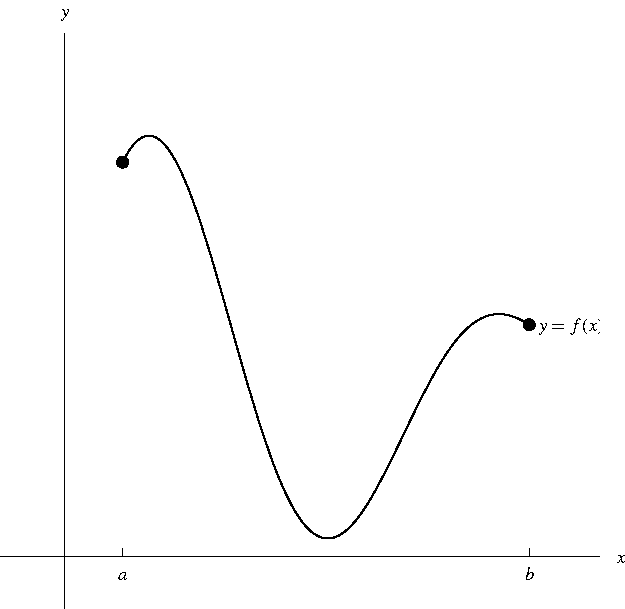
\includegraphics[height=4.5cm]{arc-length/pictures/09-01-arclengtha.pdf}%
%}%
%\only<handout:0| 2-4>{%
%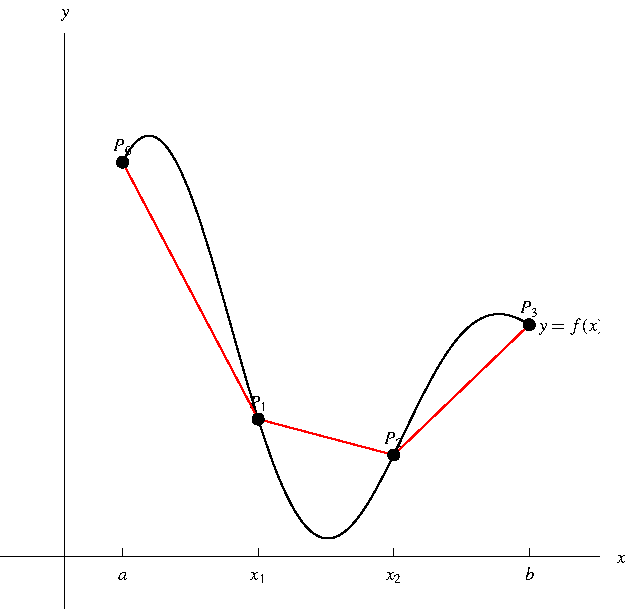
\includegraphics[height=4.5cm]{arc-length/pictures/09-01-arclengthb.pdf}%
%}%
%\only<handout:0| 5>{%
%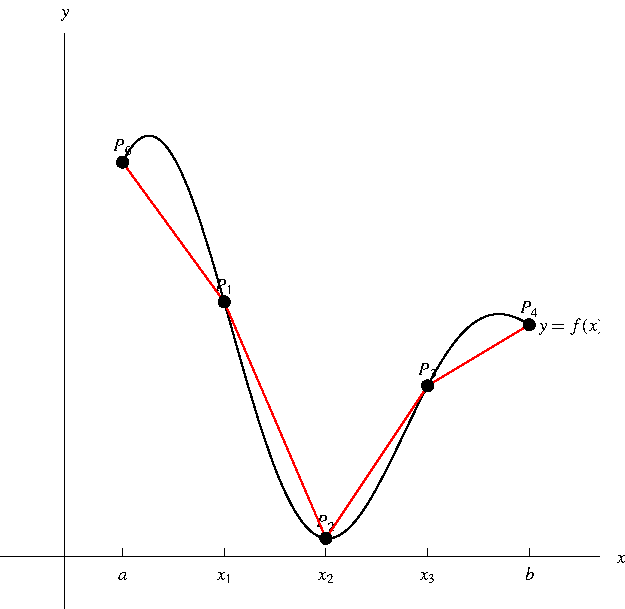
\includegraphics[height=4.5cm]{arc-length/pictures/09-01-arclengthc.pdf}%
%}%
%\only<handout:0| 6>{%
%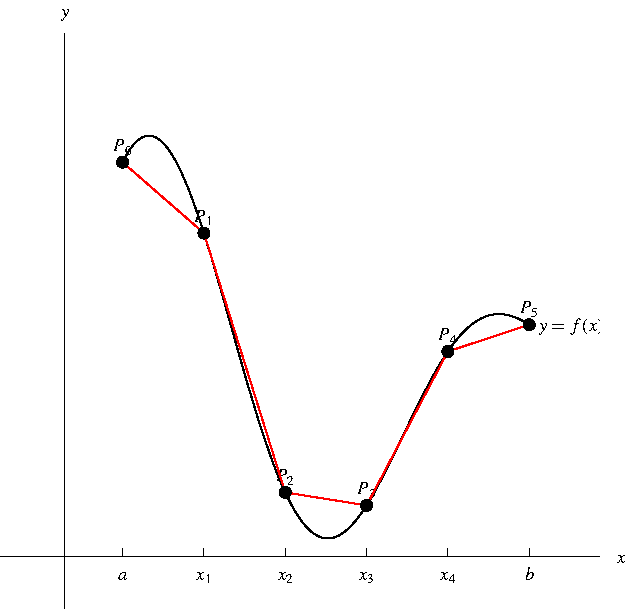
\includegraphics[height=4.5cm]{arc-length/pictures/09-01-arclengthd.pdf}%
%}%
%\only<handout:0| 7>{%
%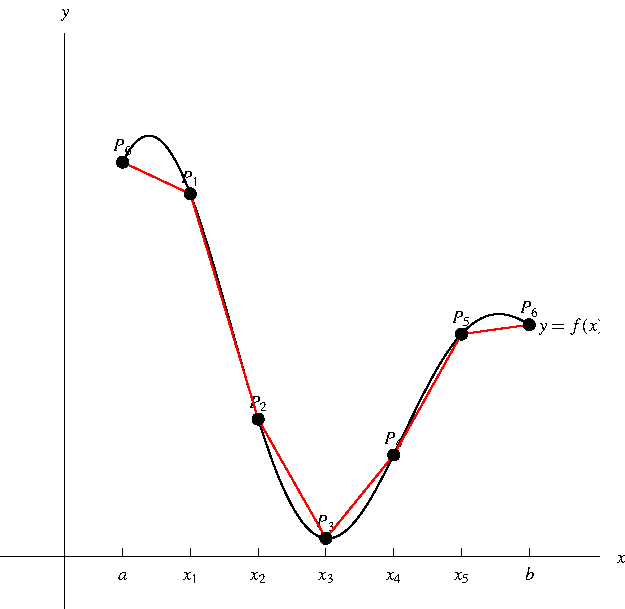
\includegraphics[height=4.5cm]{arc-length/pictures/09-01-arclengthe.pdf}%
%}%
%\only<8>{%
%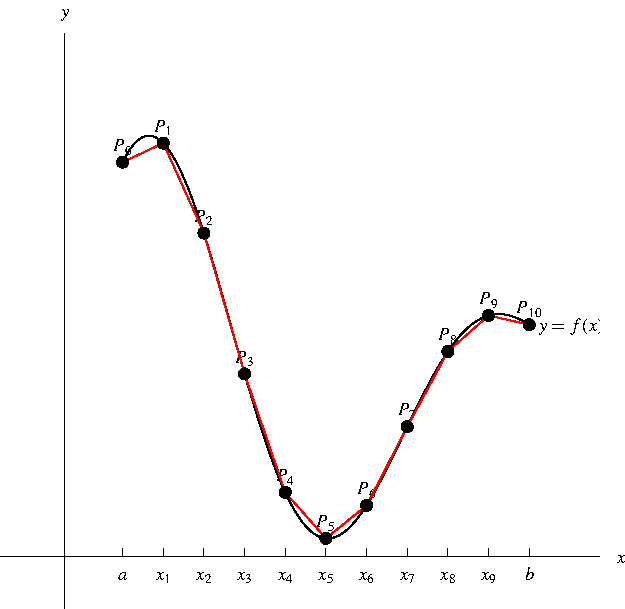
\includegraphics[height=4.5cm]{arc-length/pictures/09-01-arclengthf.pdf}%
%}%
%\only<handout:0| 9->{%
%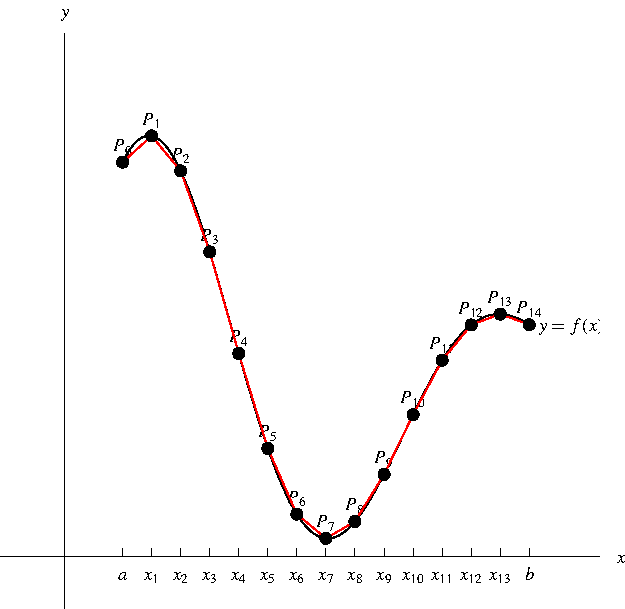
\includegraphics[height=4.5cm]{arc-length/pictures/09-01-arclengthg.pdf}%
%}%
%\only<10->{%
%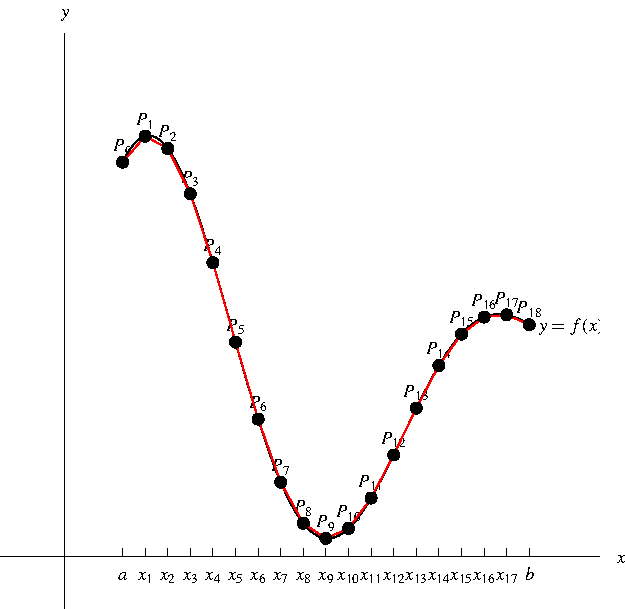
\includegraphics[height=4.5cm]{arc-length/pictures/09-01-arclengthh.pdf}%
%}%
\end{center}
\column{.4\textwidth}
\uncover<10->{%
\[
L = \lim_{n\rightarrow \infty} \sum_{i=1}^n |P_{i-1}P_i|
\]
}%
\end{columns}
\end{frame}



\begin{frame}
Let $\gamma $ be the curve
$ \gamma: \left|
\begin{array}{rcl}
x=x(t)\\
y=y(t)
\end{array}, t\in [a,b]
\right.$

$\begin{array}{rcl}
\uncover<1->{%
L = \lim_{n\rightarrow \infty} \sum_{i = 1}^n \alert<handout:0| 10>{|P_{i-1}P_i|}%
}%
& \uncover<10->{ = } &%
\uncover<10->{%
\alert<handout:0| 12>{\lim_{n\rightarrow\infty} \sum_{i=1}^n} \alert<handout:0| 10>{\sqrt{\alert<handout:0|13>{ (x'(s_i))^2}+\alert<handout:0| 13>{(y'(r_i))^2}}\ \alert<handout:0| 14>{\Delta t}}%
}\\%
& \uncover<11->{ = } &%
\uncover<11->{%
\alert<handout:0| 12>{\int_a^b} \sqrt{ \alert<handout:0| 13>{(x'(t))^2} +\alert<handout:0| 13>{(y'(t))^2}} \ \alert<handout:0| 14>{\diff t}%
}%
\end{array}
$
\begin{itemize}
\item  When $f$ has a continuous derivative we can compute arc length directly using the above limit.
\item<2->  Let $y_i = y(t_i)$, and $\Delta y = y_i - y_{i-1} = y(t_i) - y(t_{i-1})$.
\item<3-| alert@6>  Then $|P_iP_{i-1}| = \sqrt{(x(t_i)-x(t_{i-1}))^2+(y(t_i) -y(t_{i-1}))^2} = \sqrt{(\Delta x)^2 + (\Delta y)^2}$.
\item<4->  Mean Value Theorem: there exist numbers $s_i$ and $r_i$ between $t_{i-1}$ and $t_i$ such that $\alert<handout:0| 5>{x(t_i) - x(t_{i-1}) = x'(s_i )(t_i- t_{i-1})}$  and $\alert<handout:0| 5>{y(t_i) - y(t_{i-1}) = y'(r_i)( t_i-t_{i-1})}$
\item<5-| alert@5,7> $\Delta x = x'(s_i)\Delta t$, $\Delta y = y'(r_i)\Delta t$.
\end{itemize}
$\begin{array}{rcl}
\uncover<6->{%
\alert<handout:0| 10>{|P_{i-1}P_i|}%
}%
& \uncover<6->{\alert<handout:0| 10>{ = }} &%
\uncover<6->{%
\sqrt{(\alert<handout:0| 7>{\Delta x})^2 + (\alert<handout:0| 7>{\Delta y})^2}%
}  \uncover<7->{ = } \uncover<7->{%
\sqrt{ (\alert<handout:0| 7>{x'(s_i)\Delta t})^2 + (\alert<handout:0| 7>{y'(r_i)\Delta t})^2}%
}\\%
& \uncover<8->{ = } &%
\uncover<8->{%
\sqrt{(x'(s_i))^2 + (y'(r_i))^2}\sqrt{(\Delta t)^2}%
}  \uncover<9->{ = } \uncover<9->{%
\alert<handout:0| 10>{\sqrt{(x'(s_i))^2 + (y'(r_i))^2}\ \Delta t }%
}\\%
\end{array}
$
\end{frame}
}% end of scoping block
%end module arc-length-derivation-parametric
